% %%%%%%%%%%%%%%%%%%%%%%%%%%%%%%%%%%%%%%%%%%%%%%%%%%%%%%%%%%%%%%%%%%%%%
% %% SpDCache %%
% OP SpMV on Reduction Cache
% %%%%%%%%%%%%%%%%%%%%%%%%%%%%%%%%%%%%%%%%%%%%%%%%%%%%%%%%%%%%%%%%%%%%%

\section{Outer-Product SpMV with a Reduction Cache}
\label{sec:spdc:opspmvonredc}

\lettrine{A}{} widely used \gls{spFormat} to compress the non-zero elements in a matrix $A$ is \acrshort{csc}~\cite{Saad2003_COO_CSR_DIA_ELL}, where $A$ is a sparse matrix of dimensions $(M, N)$ with a number of non-zero elements $\mathit{nnz}$.
As seen in Chapter~\ref{cha:background}, it consists of three tables ($\mathit{val}$, $\mathit{idx}$, $\mathit{ptr}$) used to store non-zero values, row indices and column positions.
When performing an \acrshort{op} \acrshort{spmv} ($A \times b = c$) with this format (Algorithm~\ref{alg:spdc:spmv_with_red}), we see that a \acrshort{red} is needed to accumulate the output vector $c$ (line~6).
Moreover, $A$ is read sequentially while $c$ is updated ``randomly''.
In fact, the \emph{key} is determined via an indirection with an access to $\mathit{idx}$.

\begin{algorithm}[htbp]
    \caption{\acrlong{op} \acrshort{spmv} -- Single Threaded}
    \label{alg:spdc:spmv_with_red}
    %
    \For(\tcp*[f]{Loop over the columns of A}){$n \in \ldb 0, N-1 \rdb$}{
        \For{$pos \in \ldb ptr_n, ptr_{n+1}-1 \rdb$}{
            $key \gets idx_{pos}$\tcp*[r]{Row index}
            $val \gets val_{pos} \times b_n$\tcp*[r]{val = A\textsubscript{key,n} $\times$ b\textsubscript{n}}
            $\mathit{RED}(key, val)$\tcp*[r]{c\textsubscript{key} += val}
        }
    }
\end{algorithm}

In memory, $A$ is stored as three dense tables, but conceptually, as we perform the \acrshort{op} multiplication, the matrix is traversed from top to bottom, then left to right.
A row in the matrix corresponds to a \emph{key}, or equivalently, a position in the output vector $c$.
In Figure~\ref{fig:spdc:spmv_on_matrix}, we show an example of a sparse matrix with a few non-zero values (\ding{192} - \ding{197}).
As we traverse the matrix, we first perform a \gls{reduction} for the value on row $\mathit{key}_{10}$, then on row $\mathit{key}_{20}$ and then $\mathit{key}_{30}$.
Each of these results in a \acrshort{red} on $c$.
As we continue, we then \gls{hit} another value \ding{196} on the row $\mathit{key}_{10}$ which must be \emph{reduced} with an existing entry \ding{192}
 (as shown on the left of Figure~\ref{fig:spdc:spmv_on_matrix}, \emph{Conceptual View}).

\begin{figure}[htbp]
    \centering
    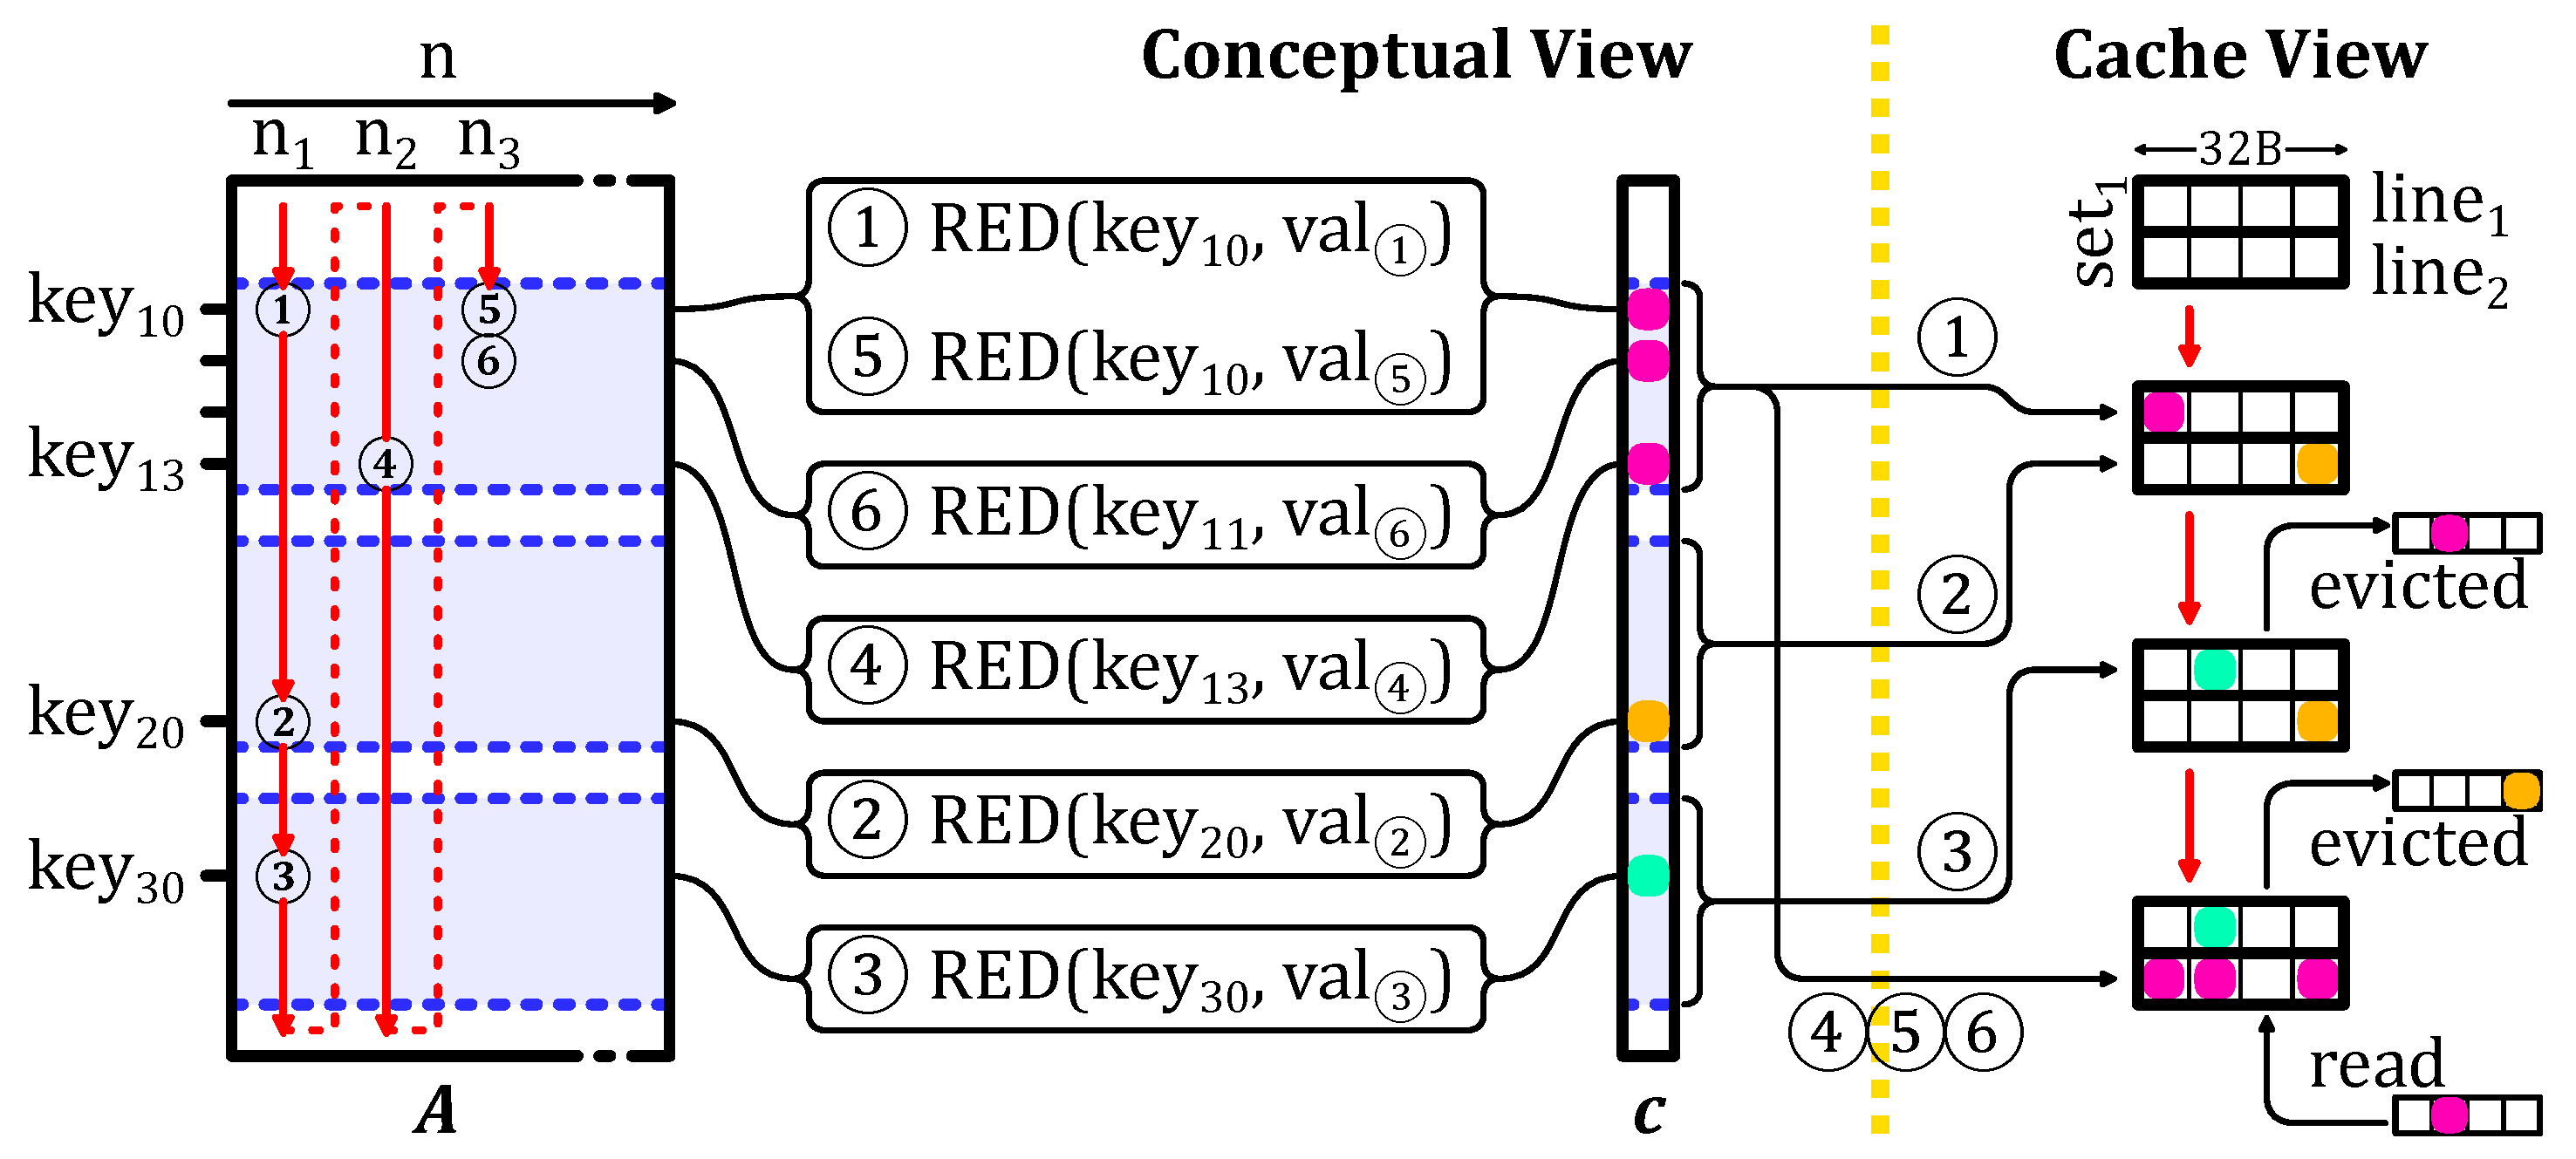
\includegraphics[width=\linewidth]{Chapter_SpDC/Figures/PDF/REDonSpMV.pdf}
    \caption{Traversal of Non-Zero Elements of Input Matrix for \acrshort{op} \acrshort{spmv} (left) and Impact on Cache (right)}
    \label{fig:spdc:spmv_on_matrix}
\end{figure}

Let us consider how $c$ is stored in a two-\gls{way} \gls{set}-associative cache with 32B lines.
We assume that all the \emph{keys} map to $\mathit{set}_1$.
When \ding{192} is updated, there is a \gls{miss} and $\mathit{line}_1$ is allocated for $\mathit{key}_{10}$.
Similarly with \ding{193}, $\mathit{line}_2$ is allocated for $\mathit{key}_{20}$.
When $\mathit{key}_{30}$ comes along, an \gls{eviction} must be performed.
We assume $\mathit{line}_1$, holding $\mathit{key}_{10}$, is evicted.
We then come to \ding{195} which has $\mathit{key}_{13}$, adjacent in memory to $\mathit{key}_{10}$, and thus stored in the same line.
This line must be brought back to process \ding{195}, \ding{196} and \ding{197}.

This example illustrates how a conventional cache can be inefficient.
First, we note the line holding $\mathit{key}_{10}$ was evicted, although it was frequently accessed after \ding{192}.
This \gls{eviction} was triggered by $\mathit{key}_{30}$, which was only accessed once.
Furthermore, for $\mathit{key}_{20}$ and $\mathit{key}_{30}$, a full line was loaded, only to modify a single entry.
A ``smarter'' cache would have maintained the line with $\mathit{key}_{10}$ to avoid an unnecessary main memory access.
Furthermore, this ``smarter'' cache would not have allocated full lines for $\mathit{key}_{20}$ and $\mathit{key}_{30}$ to only modify a single word.

The globally low local and temporal localities avoid caches, and even \glspl{redC}, to take advantage of any reuse opportunity.
However, sparse matrices have various types of structure which can have reuse potential on some parts of the matrix.
In the example in Figure~\ref{fig:spdc:spmv_on_matrix}, the first rows (on $\mathit{key}_{10}$ to $\mathit{key}_{13}$) are denser than the rest of the matrix.
A ``smarter'' cache would prefer to focus on these rows, keeping the corresponding cache-line and accumulating every elements before a final \gls{eviction}.
On the contrary, the sparser rows of the matrix would not stayed long in the ``smarter'' cache, having low priority to avoid thrashing data from denser regions.

We focus on the case of \gls{banded} matrices which have a denser region around the diagonal.
For a \gls{redC} to work efficiently with such matrices, the dense \gls{band} should be prioritized, and the isolated elements out of the band should be processed separately to avoid disturbance.
This is the main idea of \acrlong{spdc} (Paper~\ref{publ:SpDC}), which is a \gls{redC} with dedicated memory regions for the in-band and out-of-band of a matrix.
We describe its behavior int the following sections.

\begin{highlight}{Conclusion}{Red}
    When computing an \textbf{\acrshort{op} \acrshort{spmv}}, a \textbf{conventional \gls{redC} is not enough} for the available cache memory to be efficiently utilized.
    Compared to the size of a cache, matrices have too large dimensions for \emph{keys} to be reused from one column iteration to an other, leading to mostly empty cache-lines being prematurely evicted.
    \bigskip \\
    We propose \textbf{\acrlong{spdc}}, a \gls{redC} with dedicated memory regions, \textbf{leveraging matrix structure} with denser and sparser regions, such as \textbf{\gls{banded} matrices}.
\end{highlight}